\documentclass[12pt]{article}

\usepackage[utf8]{inputenc}
\usepackage{amsmath}
\usepackage{fancyhdr}
\usepackage{graphicx}
\usepackage{vmargin}
\usepackage{chemfig}
\usepackage{tikz}
\usepackage{pgfplots}
\usepackage{listings}
\usepackage{pythonhighlight}
\usetikzlibrary{snakes}

%%%%%%%%%%%%%%%%%%%%%%%%%%%%%%%%%%%%%%%%%%%%%%%%%%%%%%%%%%%%%%%%%%%%%%%%%%

\setmarginsrb{3 cm}{2.5 cm}{3 cm}{2.5 cm}{1 cm}{1.5 cm}{1 cm}{1.5 cm}
\pagestyle{fancy}
\fancyhf{}
\rhead{Jeppe Møldrup}
\chead{Studieretnings Opgave}
\lhead{22/06-2018}
\rfoot{side \thepage}
\renewcommand{\contentsname}{Indholdsfortegnelse}
\renewcommand{\baselinestretch}{1.5}

%%%%%%%%%%%%%%%%%%%%%%%%%%%%%%%%%%%%%%%%%%%%%%%%%%%%%%%%%%%%%%%%%%%%%%%%%%

\begin{document}

\begin{abstract}
This thesis is made to examine how air resistance affects a cupcake mold that is falling
through the air. Equipped with knowledge about differential calculus, velocity, acceleration
and the theory behind air resistance i have made an experiment in which i have recorded
cupcake molds falling through the air with varying masses. I have then used the collected
data to deduce an equation for calculating the air resistance that is affecting the cupcake
mold. I have used this equation in a piece of code writtin in python which creates some
ideal data for a falling cupcake mold, which i can then use to compare to the real world
data that i have recorded.
\end{abstract}
\pagebreak

\tableofcontents
\pagebreak

\section{Indledning}
I denne opgave vil jeg undersøge luftmodstandens indvirkning på en kageform gennem forsøg
hvor jeg vil indsamle data på en kageform der falder gennem luften. Udfra viden om
Differenskvotient, Differentialkvotient, hastighed, acceleration og teorien bag
luftmodstand, vil jeg med forsøget finde en ligning for luftmodstand og køre den
gennem en simulation skrevet i python og derefter sammenligne det med data fra forsøget,
for at se hvor præcist mit data er. Sammenligning giver så indblik i hvor troværdig mit data
og min ligning for luftmodstand er.

\section{Redegørelse}
Differenskvotient er sekantens hældning af to punkter $x_{0}$ og $x_{0}+\Delta x$ på en differentiabel graf.
Differentialkvotient er så tangentens hældning af et punkt $x_{0}$ på en differentiabel graf.\\
Se bilag 1.\\
Hastighed er den udledte funktion fra en stedfunktion dvs. en graf for tid og strækning, hvor den udledte funktion er en graf for tid og strækning per tid. Så hastighed er ændringen af hastighed per tid og har enheden $\frac{m}{s}$.
Acceleration er så den udledte funktion fra en hastighedsfunktion. Dvs. at acceleration er ændringen af hastighed per tid og har enheden $\frac{m}{s^2}$.\\
Teorien bag luftmodstand er at jo større tværsnitsarealet eller frontarealet for et legeme er og jo hurtigere legemet bevæger sig gennem luften, desto større er den luftmodstand der virker på legemet. Luftmodstanden vil være en kraft der peger den anden retning end den retning som legemet bevæger sig,
fordi legemet skubber luften i den retning legemet bevæger sig og så ifølge newtons tredje lov bliver legemet så udsat for en kraft der er lige så stor men omvendt af den legemet udsætter luften for.


\section{Forsøg med kageform}
Formålet med forsøget er at finde en sammenhæng mellem faldhastighed af et legeme og luftmodstanden. Forsøget går så ud på at vi lader nogle papir muffinforme falde gennem luften
hvor vi så måler papirformene med en bevægelsesføler. For at få noget variation ændrer vi på massen af papirformene ved at stakke flere papirforme oveni hinanden og lade dem falde sammen.\\
Teorien bag det er at kageformene bliver udsat for 2 kræfter. Tyngdekraften og luftmodstanden. Og når kageformene så når et punkt hvor de falder med konstant hastighed, ved vi fra newtons 1. lov
at summen af alle kræfter er lig 0. Og da luftmodstanden i dette tilfælde laver en kraft der er omvendt af tyngdekraften ved vi at de to krafter må være lig med hinanden hvir kageformen falder med
en konstant hastighed.\\
Se bilag 8.

\subsection{Ligning for $F_{luft}$}
For at finde en ligning for $F_{luft}$ starter vi med at måle en hel masse data
med kageformene. Her finder vi så et område i vores data hvor vi kan se at kageformen
falder med konstant hastighed se det gule område i bilag 7. De kan vi se fordi stedfunktionen er lineær og derfor er
den udledte funktion konstant. Så skriver vi så dataet ned i tabellen nedenunder
\begin{center}
  \begin{tabular}{| c | c | c | c | c | c | c | c | c |}
        \hline
        $v(\frac{m}{s})$ & $0.981$ & $1.14$ & $1.67$ & $2.59$ & $1.65$ & $3.05$ & $1.89$ & $1.99$ \\
        \hline
        $m(g)$ & $6.91$ & $14.07$ & $34.83$ & $62.04$ & $23.97$ & $69.51$ & $28.68$ & $40.47$ \\
        \hline
  \end{tabular}
\end{center}

Som jeg forklarede i redegørelsen for forsøget ved vi at når hastigheden er konstant. Og det kun er tyngdekraften og luftmodstanden der virker på kageformen
så vil tyngdekraften og luftmodstanden være lige store. Så vi bruger formlen
$$F_{t}=m \cdot a$$
Til at finde størrelsen på tyngdekraften der virker på kageformen. \\
Og da $F_{t}=F_{luft}$(Vi kigger kun på størrelsen af kraften her, da det er den der er ens)
kan vi bare indsætte værdierne in i tabellen nedenunder
\begin{center}
  \begin{tabular}{| c | c | c | c | c | c | c | c | c |}
        \hline
        $v(\frac{m}{s})$ & $0.981$ & $1.14$ & $1.67$ & $2.59$ & $1.65$ & $3.05$ & $1.89$ & $1.99$ \\
        \hline
        $m(g)$ & $6.91$ & $14.07$ & $34.83$ & $62.04$ & $23.97$ & $69.51$ & $28.68$ & $40.47$ \\
        \hline
        $F_{luft}(N)$ & $0.068$ & $0.138$ & $0.342$ & $0.609$ & $0.235$ & $0.683$ & $0.282$ & $0.397$ \\
        \hline
  \end{tabular}
\end{center}

Herefter indsætter vi værdierne for hastighed og luftmodstand ind i et CAS program og udfører potensregression for at finde en sammenhæng mellem
hastigheden af kageformen og luftmodstanden. Grunden til at vi bruger potensregression og ikke nogle af de andre er fordi det er den regressionstype der passer bedst med vores data.\\
Se bilag 2.
\subsection{Differentialligning}
Nu hvor vi har en formel for luftmodstand vil vi gerne kunne bruge den i en simulation så vi kan sammenligne noget af vores data med den. Den data
vi vil sammenligne med simulationsdataen er noget af det data hvor kageformen endnu ikke har ramt konstant hastighed endnu. Se bilag 7.\\
Nogle ting vi ved er
$$F_{t}=m \cdot g$$
Og den teoretiske formel for luftmodstand er
$$F_{luft}=-k \cdot v^2$$
Så
$$F_{res}=F_{luft}+F_{t}=-k \cdot v^2 + m \cdot g$$
(Dette gælder kun fordi vores akse peger nedad. Dvs. at tyngdekraften er positiv og luftmodstanden er negativ)\\
Newtons anden lov siger at
$$F_{res}=m \cdot a$$
Så vi kan substituere $F_{res}$ i den anden formel
$$-k \cdot v^2 + m \cdot g = m \cdot a$$
Så isolerer vi acceleration i formlen
$$a = \frac{-k \cdot v^2}{m} + g$$
Og som jeg forklarede i redegørelsen så er acceleration bare den udledte funktion af hastighed, så vi kan substituere
$a$ med $v'$
$$v'=\frac{-k}{m}\cdot v^2 + g$$
Og så ser vi at det er en differentialligning vi har gang i her.

\subsection{Numerisk løsning af differentialligningen}
Vi er ikke i stand til bare at finde en løsning til differentialligningen, så i stedet så løser vi den numerisk ved hjælp af Eulers metode.\\
Eulers metode er en metode hvor vi kan finde et løsning som er tæt på den rigtige løsning til differentialligningen men den er ikke den eksakte løsning.\\
Det vi gør når vi bruger Eulers metode er at vi i stedet for at udregne en funktion som er løsning til differentialligningen så tager vi en eller anden start
værdi for sted, hastighed og acceleration og tager små skridt hvor vi udregner nye værdier efter et eller andet tidsskridt.
Så i stedet for at finde den eksakte løsning, laver vi bare små bidder af lineære grafer og sætter dem sammen da vi meget nemt ud fra differentialligningen kan udregne hældningen til punkterne.\\
For at lave grafen over hastigheden vil vi så tage en starthastighed $v_0$ og lægge hældningen gange med den tid der er gået til for at få det næste punkt i vores graf. Og da vi lige har udledt
ligningen
$$v'=\frac{-k}{m}\cdot v^2 + g = a$$
vil vi finde næste punkt med formlen
$$v_{ny}=v_{gammel}+a_{gammel} \cdot \Delta t$$
Og ligeledes ville punkterne til grafen for stedet være beregnet med formlen
$$s_{ny}=s_{gammel}+v_{gammel} \cdot \Delta t$$
Da hastigheden er stedfunktionens hældning.
For at finde punkterne til accelerationen bruger vi bare differentialligningen med de gamle værdier for hastigheden
$$a_{ny}=\frac{-k}{m} \cdot v_{gammel}^2+g$$
(Her ville vi så ikke bruge den teoretiske formel for luftmodstand, men snarre den som vi selv har beregnet i forsøget med kageformene)\\
Det ville være lidt bøvlet at skulle lave alle værdierne for stedet hastigheden og accelerationen i hånden. Så vi implementerer det her i sproget Python og får vores computer til at gøre det for os
i stedet.\\
Se bilag 3.

\subsection{Sammenligning mellem forsøg og numerisk løsning}
Nu når vi så har kørt Python koden og lavet de tre diagrammer i bilag 4, 5 og 6. Kan vi så sammenligne dem med hinanden.
(Rød farve er simulationen og blå farve er vores målte data)\\
Når man kigger på grafen for sammenhængen mellem tid og sted så kan man se at den faktisk passer nogenlunde fornuftigt med dataen fra simulationen.
Men hvis man derimod kigger på graferne for sammenhængen mellem ted og hastighed og for sammenhængen mellem tid og acceleration. Så ser man at de ikke
passer lige så godt som de andre. Punkterne i de to grafer stikker kun i samme retning som dataen for simulationen men ellers er der ikke så meget til fælles for dem.
Og det skyldes fejlkilder.
Fejlkilder der indgår i vores forsøg er f.eks. at vores bevægelsesføler ikke måler hastighed eller acceleration, men i stedet regner dem ud ud fra stedfunktionen.
Så hvis stedfunktionen som føleren har målt ikke er helt god. Så bliver de resulterende hastigheds- og accelerationsfunktioner heller ikke helt gode og nok kommer til
at have relativ stor afvigelse. Derudover har vi i vores forsøg kommet til at indstille vores føler til kun at tage data med 20 hz, i stedet for at indstille den til
25 hz. Mindre datapunkter betyder normalt også at det bliver mindre præcist. Ellers er der fejlkilder som at frontarealet ikke konstant fordi vi hele tiden trækker og
skubber i kageformen uden at tænke over det, men altså på den måde skabe en afvigelse i frontarealet.

\section{Konklusion}
I denne opgave har jeg undersøgt luftmodstandens indvirkning på en kageform gennem forsøg
hvor jeg har indsamlet data på en kageform der falder gennem luften. Jeg har så
brugt denne data til at opskrive en model for luftmodstandens indvirkning. Jeg har så
brugt modellen sammen med newtons 2. lov til at opskrive en differentialligning.
Differentialligningen var i dette tilfælde ikke mulig at løse på normal vis, så
i stedet brugt jeg Eulers metode til at finde en numerisk løsning på
differentialligningen. Derefter sammenlignede jeg noget af mit opsamlede data
og så min numeriske løsning på differentialligningen. Jeg kan så konkludere at mit
data og min ligning for luftmodstand ikke er super præcise pga. fejlkilder.

\section{Bilag}
\subsection*{Bilag 1}
\begin{center}
  \includegraphics[width=\linewidth]{tangentogsekant.png}
\end{center}
Fra:\\ http://www.buhlweb.dk/matwiki/index.php?n=MatematikB.Differentialkvotient\\
Sidst besøgt: 21/06-2018 klokken 21:12

\subsection*{Bilag 2}
\begin{center}
\includegraphics[width=\linewidth]{Ligningforluftmodstand.png}
\end{center}

\subsection*{Bilag 3}
\begin{python}
  from pylab import*
  from math import*

  # --- STARTBETINGELSER ---
  s0 = 0         # Kuglen starter 5.00 meter over jorden
  t0 = 0         # Tiden er 0 s ved start
  a0 = 4.21      # Startaccelerationen er 9.82 m/s^2 - nedad!
  v0 = 0.54          # Starthastigheden er 0 m/s
  q = 1.9517759055
  k = 0.092171751618
  m = 0.03483
  g = 9.82

  dt = 0.001      # Laengden af tidsskridtet

  tidraw = [0.55, 0.6, 0.65, 0.7, 0.75, 0.8, 0.85, 0.9]
  tidboi = []
  velocityraw =[-0.54,-0.76,-0.96,-1.12,-1.25,-1.37,-1.48,-1.58]
  velocity = []
  accelerationraw = [-4.21,-4.06,-3.57,-3.01,-2.55,-2.27,-2.10,-1.78]
  acceleration = []
  positionraw = [0.85, 0.81, 0.77, 0.72, 0.66, 0.59, 0.52, 0.44]
  position = []

  for x in range(0, positionraw.__len__()):  #behandling af det raa data saa position, accelleration og hastighed stiger og starter ved 0 mens tiden starter ved 0.
      position.append(positionraw[0]-positionraw[x])
      tidboi.append(tidraw[x]-tidraw[0])
      velocity.append(-1*velocityraw[x])
      acceleration.append(-1*accelerationraw[x])

  tmax = tidboi[-1]   #saetter max tiden til den tid hvor vores data stopper.

  # --- DATA ---
  sdat = [s0]       # Liste med data - sted
  tdat = [t0]       # Tid
  vdat = [v0]       # Hastighed
  adat = [a0]     # Acceleration

  # --- Eulers metode ---
  while(t0<tmax):     # Proceduren gentages indtil makstiden opnaas
      s1 = s0 + v0*dt # Her skriver vi ligningerne ind.
      v1 = v0 + a0*dt
      p = float(math.pow(v0, q))
      a1 = float((-(k/m)*p)+g)       # Den er her konstant
      t1 = t0 + dt
      sdat.append(s1) # Beregningen af det nye punkt tilfoejes til listerne
      vdat.append(v1)
      adat.append(a1)
      tdat.append(t1)
      s0 = s1         # Det ny punkt laves til udgangspunkt for naeste beregning
      v0 = v1
      t0 = t1
      a0 = a1

  # --- GRAFIK ---
  figure(1)
  title("Sammenhaeng mellem tid og sted")
  xlabel(" t ")
  ylabel(" s ")
  plot(tdat,sdat,'ro')    # Her tegnes simuleringen
  plot(tidboi, position,'bo')    # Her tegnes simuleringen

  figure(2)
  title("Sammenhaeng mellem tid og hastighed")
  xlabel(" t ")
  ylabel(" v ")
  plot(tdat,vdat,'ro')    # Her tegnes simuleringen
  plot(tidboi,velocity,'bo')    # Her tegnes simuleringen

  figure(3)
  title("Sammenhaeng mellem tid og acceleration")
  xlabel(" t ")
  ylabel(" a ")
  plot(tdat, adat,'ro')    # Her tegnes simuleringen
  plot(tidboi, acceleration,'bo')    # Her tegnes simuleringen

  show()                  # Og her laver programmet grafen

\end{python}

\subsection*{Bilag 4}
\begin{center}
\includegraphics[width=\linewidth]{sted.png}
\end{center}

\subsection*{Bilag 5}
\begin{center}
\includegraphics[width=\linewidth]{hastighed.png}
\end{center}

\subsection*{Bilag 6}
\begin{center}
\includegraphics[width=\linewidth]{acceleration.png}
\end{center}

\subsection*{Bilag 7}
\begin{center}
\includegraphics[width=\linewidth]{maalthastighed.png}
\end{center}

\subsection*{Bilag 8}
\begin{center}
  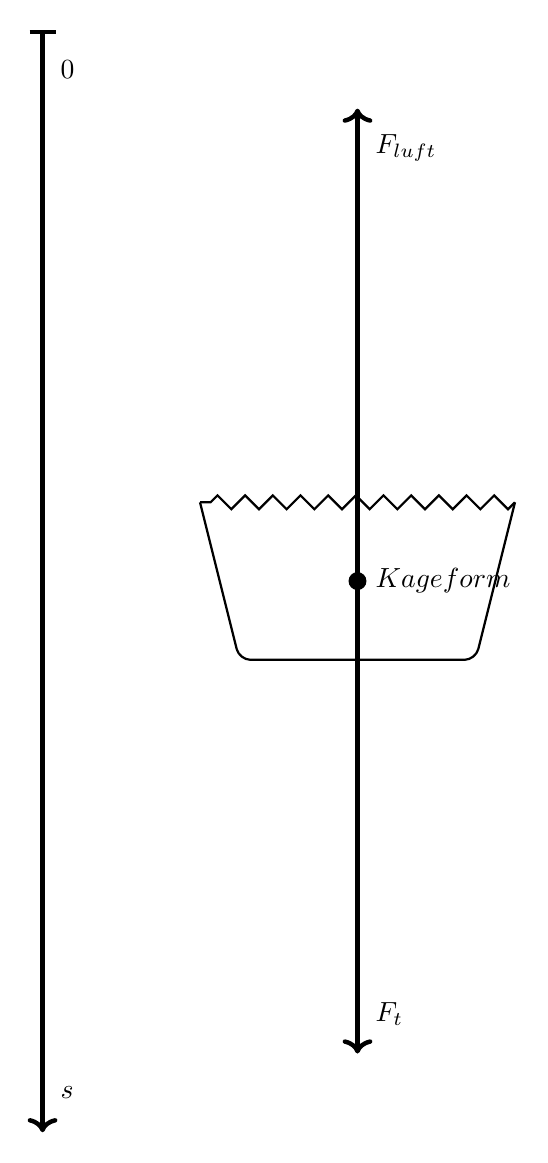
\begin{tikzpicture}[thick]

  \draw[rounded corners] (0, 3) -- (0.5, 1) -- (3.5, 1) -- (4, 3);
  \draw[snake=zigzag]  (4, 3) -- (0, 3);
  \node[draw,circle,inner sep=2pt,fill] at (2, 2) {};
  \node[anchor=west] at (2.1, 2) {$Kageform$};
  \draw[->, ultra thick] (2, 2) -- (2, 8);
  \node[anchor=west] at (2.1, 7.5) {$F_{luft}$};
  \draw[->, ultra thick] (2, 2) -- (2, -4);
  \node[anchor=west] at (2.1, -3.5) {$F_{t}$};

  \draw[|->, ultra thick] (-2, 9) -- (-2, -5);
  \node[anchor=west] at (-1.9, 8.5) {$0$};
  \node[anchor=west] at (-1.9, -4.5) {$s$};

\end{tikzpicture}

\end{center}

\end{document}
